\vspace{10pt}

{\centering\subsection*{何以萱:我的植物朋友}}

\addcontentsline{toc}{subsection}{何以萱:我的植物朋友}

\renewcommand{\leftmark}{何以萱:我的植物朋友}

\begin{figure}[htbp]

\centering

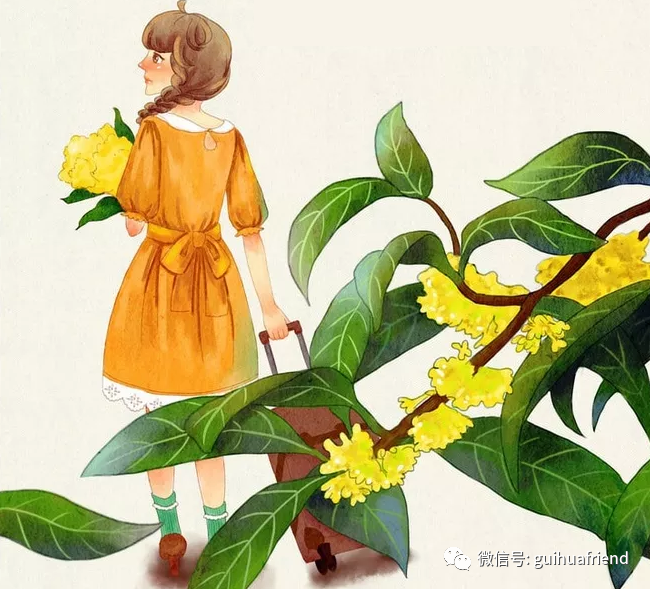
\includegraphics[width = .5\textwidth]{./ch/20.jpg}

\end{figure}



我的植物朋友是桂花,因为校园里有桂花,我家庭院里有桂花,上学的路上也有桂花,我每天都要跟桂花打招呼,所以桂花成了我的好朋友。

春天,阳光灿烂,和风细雨滋润了大地。桂花树争先恐后地长出了新叶子。它的新叶子原先是红色的,后来慢慢变绿,过了一个月以后,变成了碧绿色。碧绿的叶子一片连着一片,桂花树就像穿上了一件崭新的绿衣裳。

夏天来了,桂花叶子长大了,变得更绿了,桂花园里绿树成荫,像绿色的海洋,广阔无边,我和小伙伴在桂花树下捉虫子,做游戏感到十分凉爽,心里特别开心。

秋天,桂花树开花了,你看,碧绿的繁枝茂叶,映衬着一簇簇米黄色的小花,那就是桂花,它形态可爱, 香气醉人,用途广泛。

桂花只有米粒大小,它们相依相偎,竞相开放,细嫩的花柄,托着四片淡黄色的花瓣,小巧纤细,却尽力往外伸展,露出黄褐色的花蕾,让人感到它是那么娇小,那么玲珑。

桂花虽小,但香气很浓,还带着丝丝甜味,那浓郁的香气弥漫在空中,沁到人们的心肺里,令人陶醉,让人舒坦。

桂花还可以做桂花糖、香料、桂花酒、桂花糕……桂花糖可以放在粥里,也可以包在元宵里,尝一口,只觉一股甜丝丝的香味,令人回味无穷,不信你也试试!





\vspace{10pt}



作者:三(3)班 何以萱



指导老师:何业平



投稿:2021年5月19日





发表:2021年5月20日






                



\vspace{10pt}

\hline



